\documentclass{article}
\usepackage{ctex}
\usepackage{tikz}
\usetikzlibrary{3d,calc}
\usepackage{tikz-3dplot}
\usepackage{tikz-3dplot-circleofsphere}

\begin{document}
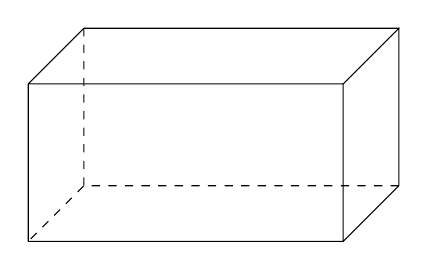
\begin{tikzpicture}[x=(-135:{0.5}),y=(0:1cm),z=(90:1cm),scale =2]
    \pgfmathsetmacro{\a}{1}
    \pgfmathsetmacro{\b}{2}
    \pgfmathsetmacro{\c}{1}

    \coordinate (A) at (\a,0,0);
    \coordinate (B) at (\a,\b,0);
    \coordinate (C) at (0,\b,0);
    \coordinate (D) at (0,0,0);
    \coordinate (A1) at (\a,0,\c);
    \coordinate (B1) at (\a,\b,\c);
    \coordinate (C1) at (0,\b,\c);
    \coordinate (D1) at (0,0,\c);

    % \foreach \x in {A,B,C,D,A1,B1,C1,D1}{
    %     \filldraw (\x)  circle (1pt) node {$\x $};
    % }
    \draw (A) -- (B)-- (C) (A1)--(B1)--(C1)--(D1)--(A1) (A)--(A1) (B)--(B1) (C)--(C1);
    \draw[dashed] (C) --(D) --(A)(D)--(D1);

\end{tikzpicture}

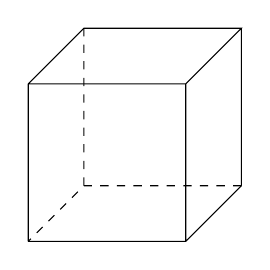
\begin{tikzpicture}[x=(-135:{0.5}),y=(0:1cm),z=(90:1cm),scale =2]
    \pgfmathsetmacro{\a}{1}
    \pgfmathsetmacro{\b}{1}
    \pgfmathsetmacro{\c}{1}

    \coordinate (A) at (\a,0,0);
    \coordinate (B) at (\a,\b,0);
    \coordinate (C) at (0,\b,0);
    \coordinate (D) at (0,0,0);
    \coordinate (A1) at (\a,0,\c);
    \coordinate (B1) at (\a,\b,\c);
    \coordinate (C1) at (0,\b,\c);
    \coordinate (D1) at (0,0,\c);

    % \foreach \x in {A,B,C,D,A1,B1,C1,D1}{
    %     \filldraw (\x)  circle (1pt) node {$\x $};
    % }
    \draw (A) -- (B)-- (C) (A1)--(B1)--(C1)--(D1)--(A1) (A)--(A1) (B)--(B1) (C)--(C1);
    \draw[dashed] (C) --(D) --(A)(D)--(D1);

\end{tikzpicture}


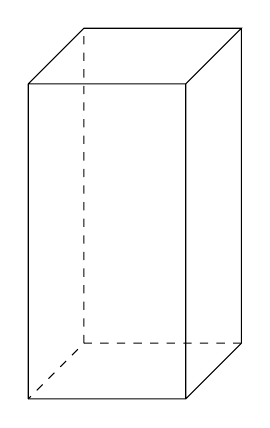
\begin{tikzpicture}[x=(-135:{0.5}),y=(0:1cm),z=(90:1cm),scale =2]
    \pgfmathsetmacro{\a}{1}
    \pgfmathsetmacro{\b}{1}
    \pgfmathsetmacro{\c}{2}

    \coordinate (A) at (\a,0,0);
    \coordinate (B) at (\a,\b,0);
    \coordinate (C) at (0,\b,0);
    \coordinate (D) at (0,0,0);
    \coordinate (A1) at (\a,0,\c);
    \coordinate (B1) at (\a,\b,\c);
    \coordinate (C1) at (0,\b,\c);
    \coordinate (D1) at (0,0,\c);

    % \foreach \x in {A,B,C,D,A1,B1,C1,D1}{
    %     \filldraw (\x)  circle (1pt) node {$\x $};
    % }
    \draw (A) -- (B)-- (C) (A1)--(B1)--(C1)--(D1)--(A1) (A)--(A1) (B)--(B1) (C)--(C1);
    \draw[dashed] (C) --(D) --(A)(D)--(D1);

\end{tikzpicture}


\def\r{1.5} \tdplotsetmaincoords{75}{110}
\begin{tikzpicture}[tdplot_main_coords,scale =2 ] \begin{scope}
\filldraw (0,0,0) circle (1pt);
\draw[tdplot_screen_coords] (0,0,0) circle (\r);
\tdplotCsDrawLatCircle{\r}{0} 
\end{scope}
% \tdplotCsDrawLatCircle[tdplotCsFront/.style={green}]{\r}{40} 
\end{tikzpicture}



\def\r{1} \def\theta{-30}\tdplotsetmaincoords{75}{110}
\begin{tikzpicture}[tdplot_main_coords,scale =2 ] 
\filldraw (0,0,0) circle (0.5pt);                     
\filldraw (0,0,{\r*sin(\theta)}) circle (0.5pt);
\draw[tdplot_screen_coords] (0,0,0) circle (\r);
\tdplotCsDrawLatCircle{\r}{\theta} 

% \tdplotCsDrawLatCircle[tdplotCsFront/.style={green}]{\r}{40} 
\end{tikzpicture}


\def\r{1} \def\theta{-30}\tdplotsetmaincoords{75}{110}
\begin{tikzpicture}[tdplot_main_coords,scale =3 ] 
\draw[tdplot_screen_coords] (0,0,0) circle (\r);
\tdplotCsDrawLatCircle{\r}{\theta} 
\coordinate (S) at (0,0,\r);
\tdplotsetcoord{A}{\r}{90-\theta}{-80}
\tdplotsetcoord{B}{\r}{90-\theta}{60}
\tdplotsetcoord{C}{\r}{90-\theta}{150}
\tdplotsetcoord{O}{0}{0}{0}
\tdplotsetcoord{O1}{{abs(\r*sin(\theta))}}{180}{0}

\foreach \i in {A,B,C,S,O,O1}
    \filldraw (\i) circle (0.5pt);

\draw (A) --(B)--(C) (S)--(A) (S)--(B) (S)--(C);
\draw[dashed] (S)--(O1) (A)--(C);

\end{tikzpicture}


\def\r{1} \def\theta{-30}\tdplotsetmaincoords{75}{110}
\begin{tikzpicture}[tdplot_main_coords,scale =3 ] 
\draw[tdplot_screen_coords] (0,0,0) circle (\r);
\tdplotCsDrawLatCircle{\r}{\theta} 
\tdplotCsDrawLatCircle{\r}{-\theta} 

\tdplotsetcoord{A}{\r}{90-\theta}{-80}
\tdplotsetcoord{B}{\r}{90-\theta}{60}
\tdplotsetcoord{C}{\r}{90-\theta}{150}
\tdplotsetcoord{A1}{\r}{90+\theta}{-80}
\tdplotsetcoord{B1}{\r}{90+\theta}{60}
\tdplotsetcoord{C1}{\r}{90+\theta}{150}
\tdplotsetcoord{O}{0}{0}{0}
\tdplotsetcoord{O1}{{abs(\r*sin(\theta))}}{180}{0}
\tdplotsetcoord{O2}{{abs(\r*sin(\theta))}}{0}{0}
\foreach \i in {A,B,C,A1,B1,C1,O2,O,O1}
    \filldraw (\i) circle (0.5pt);

\draw (A) --(B)--(C) (A1) --(B1)--(C1)--(A1) (A1)--(A) (B1)--(B) (C1)--(C);
\draw[dashed] (O2)--(O1) (A)--(C);
\end{tikzpicture}


\def\r{1} \def\theta{-20}\tdplotsetmaincoords{75}{110}
\begin{tikzpicture}[tdplot_main_coords,scale =3 ] 
\draw[tdplot_screen_coords] (0,0,0) circle (\r);
\tdplotCsDrawLatCircle{\r}{\theta} 
\tdplotCsDrawLatCircle{\r}{-\theta} 
\def\alpha{-40}
\tdplotsetcoord{A}{\r}{90-\theta}{0+\alpha}
\tdplotsetcoord{B}{\r}{90-\theta}{90+\alpha}
\tdplotsetcoord{C}{\r}{90-\theta}{180+\alpha}
\tdplotsetcoord{D}{\r}{90-\theta}{270+\alpha}
\tdplotsetcoord{A1}{\r}{90+\theta}{0+\alpha}
\tdplotsetcoord{B1}{\r}{90+\theta}{90+\alpha}
\tdplotsetcoord{C1}{\r}{90+\theta}{180+\alpha}
\tdplotsetcoord{D1}{\r}{90+\theta}{270+\alpha}
\tdplotsetcoord{O}{0}{0}{0}
% \tdplotsetcoord{O1}{{abs(\r*sin(\theta))}}{180}{0}
% \tdplotsetcoord{O2}{{abs(\r*sin(\theta))}}{0}{0}
\foreach \i in {A,B,C,D,A1,B1,C1,O,D1}
    \filldraw (\i) circle (0.5pt)
    % node {$\i$}
    ;
\draw (A) --(B)--(C) (A1) --(B1)--(C1)--(D1)--(A1) (A1)--(A) (B1)--(B) (C1)--(C);
\draw[dashed]  (A)--(C1) (A)--(D)--(D1) (C)--(D);
\end{tikzpicture}


\def\r{1} \def\theta{-20}\tdplotsetmaincoords{75}{110}
\begin{tikzpicture}[tdplot_main_coords,scale =3 ] 
\draw[tdplot_screen_coords] (0,0,0) circle (\r);
\tdplotCsDrawLatCircle{\r}{\theta} 
\tdplotCsDrawLatCircle{\r}{-\theta} 
\def\alpha{-40}
\tdplotsetcoord{A}{\r}{90-\theta}{0+\alpha}
\tdplotsetcoord{B}{\r}{90-\theta}{90+\alpha}
\tdplotsetcoord{C}{\r}{90-\theta}{180+\alpha}
\tdplotsetcoord{D}{\r}{90-\theta}{270+\alpha}
\tdplotsetcoord{A1}{\r}{90+\theta}{0+\alpha}
\tdplotsetcoord{B1}{\r}{90+\theta}{90+\alpha}
\tdplotsetcoord{C1}{\r}{90+\theta}{180+\alpha}
\tdplotsetcoord{D1}{\r}{90+\theta}{270+\alpha}
% \tdplotsetcoord{O}{0}{0}{0}
% \tdplotsetcoord{O1}{{abs(\r*sin(\theta))}}{180}{0}
% \tdplotsetcoord{O2}{{abs(\r*sin(\theta))}}{0}{0}
\foreach \i in {A,B,C,D,A1,B1,C1,D1}
    \filldraw (\i) circle (0.5pt)
    % node {$\i$}
    ;
\draw[dashed] (A) --(B)--(C) (A1) --(B1)--(C1)--(D1)--(A1) (A1)--(A) (B1)--(B) (C1)--(C);
\draw[dashed]   (A)--(D)--(D1) (C)--(D);
\end{tikzpicture}




\end{document}